%!TEX encoding = IsoLatin
%!TEX main = ../../main.tex

This chapter provides an overview of the Self-Sovereign-Identity ecosystem and Keystone Enclave framework.

\section{Self-Sovereign-Identity}
Self-Sovereign Identity (SSI) \cite{tobin2016inevitable} is a new model for digital identity. In the SSI ecosystem, a user can fully control his own identity and use it between any service. SSI is different from today's digital identities: it is anchored to distributed ledgers so is not controlled by any centralized services.
One SSI innovation is the design and development of a common set of specifications: 
Decentralized Identifiers (DIDs) \cite{didW3C} and Verifiable Credentials (VCs) \cite{vcW3C}, by doing this a user identity can be anchored to different distributed ledgers but it will be defined in the same standard way.

\subsection{Decentralized Identifiers}  
DIDs \cite{didW3C} are identifiers referring to any subject determined by the controller of the DID.
A DID's controller can demonstrate control over it thanks to the design without requesting permission from any other party allowing a verifiable, decentralized digital identity, that will be independent of identity providers, and certification authorities.

\subsubsection*{Overview}

In detail a DID is a type of URI \cite{berners2005uniform} scheme that links a DID subject with a DID document allowing trustable interactions associated with that subject. The subject of a DID is the entity identified by the DID and can be a person, a group or an organization. Typically the DID subject is also the controller, but a DID can have more than one. 

Specifically, a DID is a simple text string, as shown in the figure \ref{didExample}, consisting of three parts: 
\begin{itemize}
    \item the DID URI scheme identifier
    \item the identifier for the DID method
    \item the DID method-specific identifier
\end{itemize}

\begin{figure}[h!]
    \centering
    \includesvg[inkscapelatex=false, scale=0.70]{./chapters/images/parts-of-a-did.svg}
    \caption{A simple example of a DID \cite{didW3C}.}
    \label{didExample}
\end{figure}

A DID resolves to a DID document, a DID document contains information about a DID subject and cryptographic material that will be used to prove control of that DID. DID documents can be represented in JSON \cite{json-rfc3986} or JSON-LD \cite{json-ld} format, as can be seen in the listing \ref{didDocExample}. Only the controller of the DID has the right to make changes to the related DID document. 

DIDs are generally stored in some underlying system or network for resolution to DID documents. A verifiable data registry is a system that enables the recording of DIDs and the return of the data required to produce DID documents. Distributed ledgers, decentralized file systems, all types of databases, peer-to-peer networks, and other trusted data storage methods are some examples. The operations to create, resolve, update, and deactivate a DID and the related DID document are defined by DID methods and their specifications, which are generally coupled with a distinct verifiable data registry \cite{didW3C}. 
A DID URL expands the syntax of a DID with other standard components of URI such as path, query, and fragment to find a specific resource, such as a cryptographic public key in a DID document or a resource outside the DID document. \\

\begin{lstlisting}[caption={Example of a simple DID document from \cite{didW3C}.},captionpos=b,style=json, label={didDocExample},frame=single]
{
    "@context": [
        "https://www.w3.org/ns/did/v1",
        "https://w3id.org/security/suites/ed25519-2020/v1"
    ]
    "id": "did:example:123456789abcdefghi",
    "authentication": [{

        "id": "did:example:123456789abcdefghi#keys-1",
        "type": "Ed25519VerificationKey2020",
        "controller": "did:example:123456789abcdefghi",
        "publicKeyMultibase": "zH3C2AVvLMv6gmMNam3uVAjZpfkcJCwDwnZn6z3wXmqPV"
    }]
}
\end{lstlisting}

\begin{figure}[h!]
    \centering
    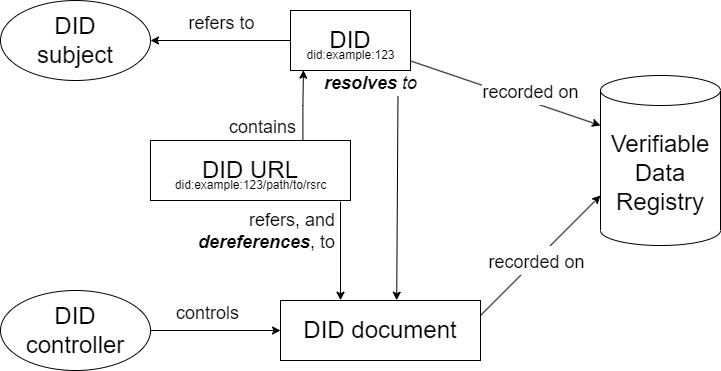
\includegraphics[width=10cm]{./chapters/images/did-overview.png}
    \caption{DID architecture overview and relationships between components \cite{didW3C}.}
    \label{didOverview}
\end{figure}

\subsection{Verifiable Credentials}
Verifiable Credential \cite{vcW3C} provides a standard method to express credentials on the internet in a way that is cryptographically safe, privacy-respecting, and machine-verifiable.
In our daily lives a credential could consist of:
\begin{itemize}
    \item information related to identifying the subject of the credential (for example, a photo, name, or identification number)
    \item information related to the issuing authority (for example, a city government or a university)
    \item information related to the type of credential this is (for example, a passport or a driving license)
    \item information related to specific attributes or properties being asserted by the issuing authority about the subject (for example, nationality, the classes of vehicle entitled to drive, or date of birth)
    \item information related to constraints on the credential (such as expiration date, or terms of use). 
\end{itemize}

In verifiable credentials, the inclusion of digital signatures makes them more trustworthy and more tamper-evident against physical credentials allowing third-party verified machine-readable personal information usable on the Web for receiving services and benefits as in the physical world \cite{vcW3C}.

\subsubsection*{Overview}

Distinct actors can be identified in the verifiable credentials ecosystem, which defines the roles and the relationships between them. The separation of roles allows the standardization of interfaces and protocols. In detail the existing entities that determine the \textit{trust triangle} \cite{trustOverIP} are: 

\begin{itemize}
    \item \textit{holder}: his role is to request, possess or use verifiable credentials. Example holders include students, employees, and customers.
    \item \textit{issuer}: his role is to create a verifiable credential and provide that to a holder by asserting claims about one or more subjects. For example, an issuer is a government. 
    \item \textit{verifier}: his role is to process verifiable credentials provided by holders. Example verifiers are whoever provides a service. 
\end{itemize}

\begin{figure}[h!]
    \centering
    \includesvg[inkscapelatex=false, scale=0.70]{./chapters/images/vc-ecosystem.svg}
    \caption{The roles and information flows of Verifiable Credential \cite{vcW3C}.}
    \label{vcEcosystem}
\end{figure}

To use verifiable credentials a holder has to generate verifiable presentations by enclosing them and signing before presenting them to a verifier, by doing this a holder demonstrates the possession of the verifiable credential. The fact that a credential is verifiable by the verifier does not mean that the claims it contains are true. Another aspect that variable credentials enhance is privacy. The usage of machine-readable credentials allows malicious actors to collect and correlate data, compromising holders' privacy. Variable credentials specification draft how to deal with these issues, by using privacy-enhancing technologies, such as \textit{zero-knowledge proofs} \cite{zkp-survey}. 

\begin{figure}[h!]
    \centering
    \includesvg[inkscapelatex=false, scale=0.45]{./chapters/images/credential.svg} 
    \hfil
    \includesvg[inkscapelatex=false, scale=0.45]{./chapters/images/presentation.svg}
    \caption{Basic components of a verifiable credential and a verifiable presentation \cite{vcW3C}.}
    \label{vc-vp-topview}
\end{figure}

Verifiable credentials and verifiable presentations can be represented in JSON \cite{json-rfc3986} or JSON-LD \cite{json-ld} format as can be seen in listings \ref{vcExample} and \ref{vpExample}. \\

\begin{lstlisting}[caption={A simple example of a verifiable credential \cite{vcW3C}.},captionpos=b,style=json, label={vcExample},breaklines=true,frame=single]
{
    "@context": [
        "https://www.w3.org/2018/credentials/v1",
        "https://www.w3.org/2018/credentials/examples/v1"
    ],
    "id": "http://example.edu/credentials/1872",
    "type": ["VerifiableCredential", "AlumniCredential"],
    "issuer": "https://example.edu/issuers/565049",
    "issuanceDate": "2010-01-01T19:23:24Z",
    "credentialSubject": {
        "id": "did:example:ebfeb1f712ebc6f1c276e12ec21",
        "alumniOf": {
            "id": "did:example:c276e12ec21ebfeb1f712ebc6f1",
            "name": [{
                "value": "Example University",
                "lang": "en"
            }]
        }
    },    
    "proof": {
        "type": "RsaSignature2018",
        "created": "2017-06-18T21:19:10Z",
        "proofPurpose": "assertionMethod",
        "verificationMethod": "https://example.edu/issuers/565049#key-1",
        "proofValue": "eyJhbGciOiJSUzI1NiIsImI2NCI6ZmFsc2UsI..."
        }
}
\end{lstlisting}

\begin{lstlisting}[caption={A simple example of a verifiable presentation \cite{vcW3C}.},captionpos=b,style=json, label={vpExample},breaklines=true,frame=single]
    {
        "@context": [
          "https://www.w3.org/2018/credentials/v1",
          "https://www.w3.org/2018/credentials/examples/v1"
        ],
        "type": "VerifiablePresentation",
        "verifiableCredential": [{
            ...
        }],
        "proof": {
          "type": "RsaSignature2018",
          "created": "2018-09-14T21:19:10Z",
          "proofPurpose": "authentication",
          "verificationMethod": "did:example:ebfeb1f712ebc6f1c276e12ec21#keys-1",
          "challenge": "1f44d55f-f161-4938-a659-f8026467f126",
          "domain": "4jt78h47fh47",
          "proofValue": "Qy72IFLN25DYuNzVBAh4vGHSrQyHUGlc..."
        }
      }   
\end{lstlisting}

\subsection{Distributed Ledgers Technologies}

Distributed Ledger Technology (DLT)  is a new paradigm for collecting and sharing information between people. A distributed ledger is a database that is spread across several nodes or computing devices. An exact copy of the ledger is replicated and stored on each node. The revolutionary aspect of distributed ledger technology is that no single administrator or central authority is responsible for maintaining the ledger. Each network's participant node keeps its state updated by constructing and recording updates to the ledger independently. The nodes then vote on these adjustments to ensure that the majority agrees with the conclusion reached. This voting and agreement on the state of the ledger is called consensus and is conducted automatically via a consensus algorithm \cite{dlt-intro-1}. 
The following criteria can be used to categorize DLTs: data structures, consensus algorithms, permissions, mining accessibility and so on. The main data structure types are blockchains and Directed Acyclic Graphs (DAGs). Although blockchains are the most popular and well-known DLT type,  DLTs based on Directed Acyclic Graph (DAG) data structures are becoming more popular because they reduce transaction data size and transaction fees, and increase transaction speeds \cite{dlt-intro-2}.

An Example of DAG DLT is the \textit{tangle} of IOTA \cite{popov2018tangle}, a cryptocurrency for the Internet-of-Things (IoT) industry.

\begin{figure}[h!]
    \centering
    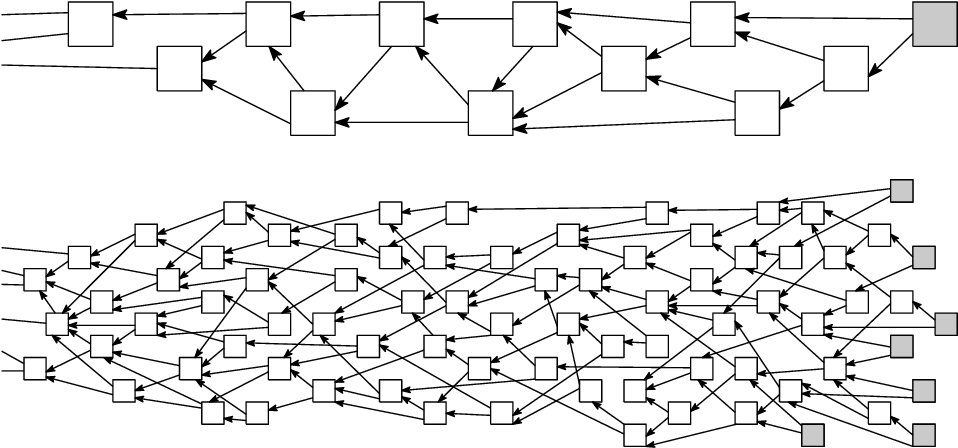
\includegraphics[width=10cm]{./chapters/images/tangle.png}
    \caption{Visualizations of the IOTA tangle \cite{popov2018tangle}.}
    \label{tangleFigure}
\end{figure}

%parlare di come è immutabile una blockchain?

\section{Keystone Enclave}
Device manufacturers are now taking security concerns more seriously than they previously did as a result of the rise in popularity of networked devices in recent years.
To adequately address these challenges, a specification has been developed that defines a way to ensure the integrity and confidentiality of sensitive data in the device that implements the specification.
\cite{IntroTEE}
\subsection{Trusted Execution Environment}
A Trusted Execution Environment (TEE) is a safe area within a CPU. It runs in an isolated environment and in parallel with the operating system.
It ensures that the confidentiality and integrity of the code and data loaded in the TEE are preserved. 
Trusted applications running on TEE have access to the full capabilities of a device's main processor and memory, while hardware isolation shields these components from user-installed apps running in the main operating system. The various included trusted applications are protected from one another by software and cryptographic isolations within the TEE.
\cite{IntroTEE}
%aggiungere definizione di enclave, tcb?
The two most common TEE implementations at the moment are ARM TrustZone and Intel SGX. All these TEEs make design decisions based on either the target applications or threat models and these choices are fixed since they are strictly hardware related. They were not designed to have flexibility or extensibility for enclave developers.  If the hardware changes or has a new feature, the enclave developer has to redesign the TEE.
All TEE platforms aim to reduce the enclave's TCB, yet they have managed to achieve different degrees of success. Additionally, closed-source hardware and microcode implementations make it impossible for a third party to evaluate the security of TEEs.



\textbf{Customizable TEE} is the solution to these problems. It has been designed to be flexible, and configurable and to have a small TCB. It has been developed with clear abstractions and a modular programming model which simplifies for others to extend and add features to the TEE. A customizable TEE is Keystone.
\cite{lee2020keystone} 
\subsection{Keystone overview}
Keystone \cite{lee2020keystone} is an open-source framework for creating RISC-V hardware-based Trusted Execution Environments (TEEs) that are adaptable for use on a variety of platforms. Keystone offers security primitives that can be joined together via the software framework rather than creating a single instance of TEE hardware. The TEE can be modified by the creator of the enclave and the platform provider to suit their threat models or platform configurations. The Keystone project offers a general and formally proven interface for a variety of devices to create an open standard for TEEs. Every piece of hardware could, in our opinion, have a secure TEE at practically no extra cost.

\begin{figure}[h!]
    \centering
    \includesvg[inkscapelatex=false, scale=0.40]{./chapters/images/TEE-keystone-vs-x86.svg}
    \caption{architecture differences between x86 and keystone}
    \label{keystone-vs-x86}
\end{figure}
\subsubsection{Security Monitor}
\subsubsection{Runtime}